\documentclass[11pt]{article}

% packages
\usepackage[margin=1in]{geometry}
\usepackage{amsmath,amssymb,amsthm}
\usepackage{booktabs}
\usepackage{xcolor}
\usepackage{graphicx}
\usepackage{float}
\usepackage{tikz}
\usetikzlibrary{arrows.meta, positioning, shapes.geometric, calc, fit, backgrounds}
\usepackage{listings}
\usepackage{algorithm2e}
\usepackage{hyperref}
\usepackage[numbers]{natbib}
\usepackage{tabularx}
\usepackage{pdflscape}
\usepackage{array}

% listings style
\lstset{
  language=Python,
  basicstyle=\ttfamily\small,
  keywordstyle=\color{blue!70!black},
  commentstyle=\color{gray},
  stringstyle=\color{orange!80!black},
  breaklines=true,
  frame=single,
  numbers=left,
  numberstyle=\tiny\color{gray},
  xleftmargin=2em,
  framexleftmargin=1.5em,
}

% theorem environment
\newtheorem{theorem}{Theorem}
\newtheorem{definition}{Definition}

% pulak's commands
\newcommand{\red}[1]{\textcolor{red}{#1}}

\title{RL-Based Memory Pooling for Octopus CXL Systems}
\author{Pulak Mehrotra}
\date{}

\begin{document}
\maketitle
\tableofcontents
\newpage

% ======================================================================
\section{Problem Formulation}
% ======================================================================

\subsubsection*{Setting: CXL-Based Memory Pooling}

Modern cloud datacenters at Microsoft deploy \emph{Compute Express Link (CXL)}
to pool DRAM across servers.  Rather than each host owning fixed local memory,
CXL exposes pooled memory devices that multiple hosts can share, allowing the
aggregate pool to be right-sized to the workload's \emph{average} demand
rather than its per-server \emph{peak}---yielding meaningful memory savings.

The \textbf{Octopus} architecture targets cost-effective CXL deployments using
\emph{Multi-Ported CXL Devices (MPDs)} instead of expensive CXL switches.
Each MPD connects to several servers, and each server connects to several MPDs,
forming a \emph{sparse bipartite graph} between hosts and memory devices
(Figure~\ref{fig:bipartite}).

\begin{figure}[H]
\centering
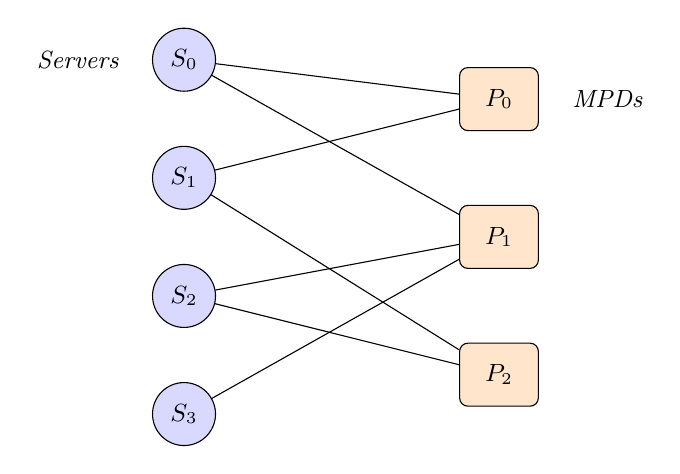
\begin{tikzpicture}[
    >=Stealth,
    node distance=1.0cm,
    every node/.style={font=\small},
    host/.style={draw, circle, fill=blue!15, minimum size=0.8cm},
    mpd/.style={draw, rectangle, rounded corners=3pt, fill=orange!20,
                minimum height=0.8cm, minimum width=1.0cm, align=center},
]
    % Hosts (left column)
    \node[host] (H0) at (0,  3)   {$S_0$};
    \node[host] (H1) at (0,  1.5) {$S_1$};
    \node[host] (H2) at (0,  0)   {$S_2$};
    \node[host] (H3) at (0, -1.5) {$S_3$};

    % MPDs (right column)
    \node[mpd]  (P0) at (4,  2.5)  {$P_0$};
    \node[mpd]  (P1) at (4,  0.75) {$P_1$};
    \node[mpd]  (P2) at (4, -1.0)  {$P_2$};

    % Sparse edges
    \draw[-] (H0) -- (P0);
    \draw[-] (H0) -- (P1);
    \draw[-] (H1) -- (P0);
    \draw[-] (H1) -- (P2);
    \draw[-] (H2) -- (P1);
    \draw[-] (H2) -- (P2);
    \draw[-] (H3) -- (P1);

    % Labels
    \node[font=\small\itshape, left=0.3cm of H0] {Servers};
    \node[font=\small\itshape, right=0.3cm of P0] {MPDs};
\end{tikzpicture}
\caption{Octopus bipartite graph: servers (left) connect to MPDs (right) via
sparse edges.  Each edge denotes a physical CXL link over which a server can
allocate memory from that MPD.}
\label{fig:bipartite}
\end{figure}

\subsubsection*{The Memory Allocation Problem}

When a VM is scheduled on host $S_i$, it requests $x$ GB of CXL memory.
Host $S_i$ can only draw from the MPDs it is physically connected to---the
set $\mathcal{N}(i)$ of its CXL neighbors.  The allocation algorithm must
decide how to split the request $x$ across those MPDs.

\begin{definition}[Memory Allocation Policy]
Let $n$ be the number of servers, $m$ the number of MPDs, and $M \in \{0,1\}^{n
\times m}$ the adjacency matrix of the bipartite CXL graph (with $M_{ij} = 1$
iff server $i$ has a link to MPD $j$).  At each VM arrival event, a
\emph{memory allocation policy} $\pi$ maps the current system state to a
non-negative allocation vector $\mathbf{a} \in \mathbb{R}_{\ge 0}^{m}$
satisfying
\[
    \sum_{j=1}^{m} a_j = x,
    \qquad
    a_j = 0 \text{ whenever } M_{ij} = 0.
\]
\end{definition}

\subsubsection*{Why Pooling Helps: The Statistical Argument}

Cloud servers are provisioned for their \emph{individual} peak demand, but
peaks across servers are not synchronized.  At any given instant, some servers
are lightly loaded while others are saturated.  If those servers share a common
pool of CXL memory, the aggregate capacity only needs to cover the
\emph{population} peak---the worst-case total demand summed over all servers at
any one moment---rather than the sum of each server's individual peak.

Concretely, Figure~5 of the Acadia paper (production VM traces from a large
cloud provider, 10 clusters, two weeks) shows that grouping 25--32 hosts still
requires $\sim 1.5\times$ average capacity to cover peak demand.  The
peak-to-average ratio decays slowly with pod size and flattens near 100 hosts,
which is why Acadia targets 96-host pods.

\subsubsection*{Objective}

The figure of merit is \emph{pooling savings}: the fraction by which CXL
capacity can be reduced relative to the total server DRAM installed in the pod.

\paragraph{Simulation model.}
The simulation replays production VM traces.  At each tick (e.g.~5~min), every
active VM contributes its allocated memory footprint to its host's demand.  When
a VM is launched, the allocation policy decides which MPD(s) supply its memory.
When the VM terminates, the capacity is released.  No migration between MPDs
is assumed.  The required CXL capacity is the \emph{peak per-MPD load}: the
single highest per-MPD usage across all MPDs and all ticks.

\paragraph{Formal objective.}
Since all MPDs in a pod are provisioned identically, the peak per-MPD load
determines the capacity---and thus the cost---of every device.

\[
    \text{Pooling Savings} = 1 -
    \frac{m \cdot \max_{j \in [m]} \; \text{PeakLoad}_j}
         {\sum_{i=1}^{n} \text{DRAM}_i},
\]

where $\text{PeakLoad}_j = \max_{t} \sum_{i : M_{ij}=1} d_i(t)$ is the maximum
total demand placed on MPD $j$ at any single time step, $m$ is the number of
MPDs, and $n$ is the number of servers.  Higher savings correspond to smaller
required CXL capacity.

\paragraph{Cost model interpretation.}
Memory constitutes roughly 50\% of server cost.  With 65\% of DRAM on MPDs
(the remainder too latency-sensitive for CXL), the Acadia cost model shows that
a 3\% pooling saving is the \emph{breakeven} point---enough to offset the extra
cost of MPDs over plain expansion devices.  The Acadia-96 topology achieves
$\approx 16\%$ savings; unrealistically large random topologies ($>512$ hosts)
plateau near 18\%, showing that 96 hosts is close to the cost-efficient frontier
under copper cabling constraints.

\paragraph{The greedy--optimal gap.}
The \textbf{greedy} policy allocates each VM's demand to the currently
least-loaded reachable MPD at arrival time and never migrates.  It is simple
and migration-free but myopic: a VM with a long lifetime placed on an MPD early
in the day may block better placements for later VMs, inflating the peak.

The \textbf{optimal} policy re-balances all allocations at every tick (allowing
full migration) and achieves the true minimum peak over the horizon.  It
requires global future knowledge and unlimited migration---impractical in
production.

The \textbf{RL agent} targets the gap: make allocation decisions \emph{at VM
arrival time}, using only the current system state and any patterns learnable
from historical traces, to minimize the peak per-MPD load without any
migration.  The key challenge is learning to anticipate future demand so that
today's placements leave headroom for tomorrow's hot spots.

\paragraph{Numerical target.}
For a 96-host Acadia pod with $m = 120$ MPDs (80 internal + 40 external) each
initially provisioned at greedy-policy capacity, beating the greedy policy by
even 1--2 percentage points in savings translates directly to a reduction in the
required per-MPD capacity and a meaningful decrease in pod CapEx at hyperscale.

\subsubsection*{Why Sparse Topologies Are Harder}

In a fully-connected topology every server can access every MPD, and a simple
load-balancing rule achieves near-optimal pooling savings.  In the sparse
Octopus topology, the graph's \emph{expansion} property governs how well
demand imbalances can be absorbed:

\begin{definition}[Graph Expansion]
For a given subset size $k$, the expansion $e_k$ of the bipartite graph is
the minimum number of distinct MPDs connected to any subset of $k$ servers.
\end{definition}

High expansion means that even a ``hot'' subset of servers---those with
simultaneously elevated memory demand---can spread their excess demand across
many MPDs.  Random and expander graphs achieve significantly better pooling
than regular low-degree graphs.

\subsubsection*{Workload Dynamics}

The allocation problem is \emph{dynamic}: VMs arrive and depart continuously,
changing per-server memory demand over time.  Critically, once a VM's memory is
allocated to an MPD, migrating that allocation to a different MPD has a
non-trivial runtime cost.  This creates a temporal coupling between past
allocation decisions and future capacity: a bad allocation today may force
avoidable fragmentation tomorrow.

This combination---sparse connectivity, dynamic demand, and migration cost---is
what makes heuristic policies suboptimal and motivates a learning-based
approach.

% ======================================================================
\section{Why is RL a Good Solution?}
% ======================================================================

\subsubsection*{Brief Introduction to Reinforcement Learning}

Reinforcement learning (RL) is a machine learning paradigm in which an
\emph{agent} interacts with an \emph{environment} over discrete time steps.
At each step the agent observes a \emph{state} $s_t \in \mathcal{S}$, selects
an \emph{action} $a_t \in \mathcal{A}$, receives a scalar \emph{reward}
$r_t \in \mathbb{R}$, and transitions to the next state $s_{t+1}$.  The agent's
goal is to learn a \emph{policy} $\pi(a_t \mid s_t)$ that maximises the
expected discounted cumulative reward,
\[
    J(\pi) = \mathbb{E}_{\pi}\!\left[\sum_{t=0}^{\infty} \gamma^t r_t\right],
\]
where $\gamma \in [0, 1)$ is a discount factor.

RL is particularly well suited to problems where:
\begin{itemize}
    \item The optimal action cannot be computed analytically (large or
          continuous state/action spaces).
    \item The environment is non-stationary or partially observable.
    \item Decisions have long-horizon consequences that are hard to capture
          with myopic heuristics.
    \item Patterns exist in the data that can be exploited with a
          learned model.
\end{itemize}

All four of these conditions hold in the Octopus memory allocation setting.

\subsubsection*{Why Standard Approaches Fall Short}

Three key properties of the problem make rule-based and classical
optimisation approaches impractical at production scale:

\begin{enumerate}
    \item \textbf{Non-stationary and partially observable workloads.}
    VM memory demand is driven by customer applications, which vary with
    time-of-day, day-of-week, and across customer segments.  A static policy
    tuned for one workload profile degrades on another.

    \item \textbf{Snowball effect of allocation.}
    An MPD that accumulates memory from several VMs early in a day becomes a
    ``hot'' device later.  Allocation decisions are therefore path-dependent:
    early choices constrain future flexibility.

    \item \textbf{Large and structured decision space.}
    With $n$ servers and $m$ MPDs, the allocation at each VM arrival is a
    continuous vector in $\mathbb{R}^m$ subject to graph-adjacency and
    capacity constraints.  Enumerating or explicitly optimising over this
    space per-event is intractable at cloud scale.
\end{enumerate}

RL side-steps these difficulties by \emph{learning} an allocation policy from
experience (VM trace replay), allowing it to implicitly encode temporal
patterns and long-horizon consequences without explicit modelling.

\subsubsection*{Precedent in Systems Research}

Learning-based resource management has a strong track record in systems:
\begin{itemize}
    \item \textbf{Pensieve} (SIGCOMM '17): RL for adaptive bitrate streaming.
    \item \textbf{Decima} (SIGCOMM '19): RL for scheduling in Spark workloads.
    \item \textbf{FleetIO} (ASPLOS '25): RL for SSD capacity allocation across
          servers---arguably the closest prior work to our setting.  FleetIO
          trains a decentralised RL agent (one per virtual SSD) that
          learns allocation directly from telemetry, without an explicit
          performance model.  Its reward balances local utilisation against
          global contention, an approach we adapt for the memory pooling
          setting.
\end{itemize}

Additionally, \textbf{Coach} (ASPLOS '25) demonstrates that VM memory
utilisation follows predictable diurnal patterns---a regularity that an RL
agent can exploit to anticipate future demand and make proactive allocation
decisions.

% ----------------------------------------------------------------------
\subsection{Data Plotting}
\label{sec:data_plotting}
% ----------------------------------------------------------------------

We use production VM traces from ten Azure datacenters, collected over a
two-week window in December 2024.  Each trace is a pre-processed pickle
containing per-VM records with start/end timestamps and memory footprint
(\texttt{rss[1]}, in GB).  Time is discretised into 5-minute ticks; at each
tick, per-server CXL demand equals the sum of \texttt{rss[1]} across all VMs
active on that server.

\subsubsection*{Raw Demand Time-Series}

Figure~\ref{fig:demand_overview} shows the cluster-aggregate memory demand
(blue) for all ten datacenters over the two-week trace window, together with
individual per-server demand curves (grey) and the cluster peak (red dashed)
and mean (green dotted).  Several patterns are immediately apparent:

\begin{itemize}
    \item \textbf{Diurnal cycling.}  Every site shows a clear 24-hour rhythm;
          demand rises during business hours and falls overnight.  The
          amplitude and phase of the cycle vary by geography (e.g.\ Amsterdam
          and London peak in European daytime; Singapore and Sydney peak
          independently).
    \item \textbf{High peak-to-mean ratio.}  The cluster peak is typically
          1.3--1.6$\times$ the mean.  This gap is the headroom that pooling
          can eliminate.
    \item \textbf{Per-server heterogeneity.}  The grey traces span a wide
          band, confirming that individual server demand is far more variable
          than the aggregate.  Pooling reduces required capacity precisely
          because these individual peaks are not synchronized.
\end{itemize}

\begin{figure}[H]
    \centering
    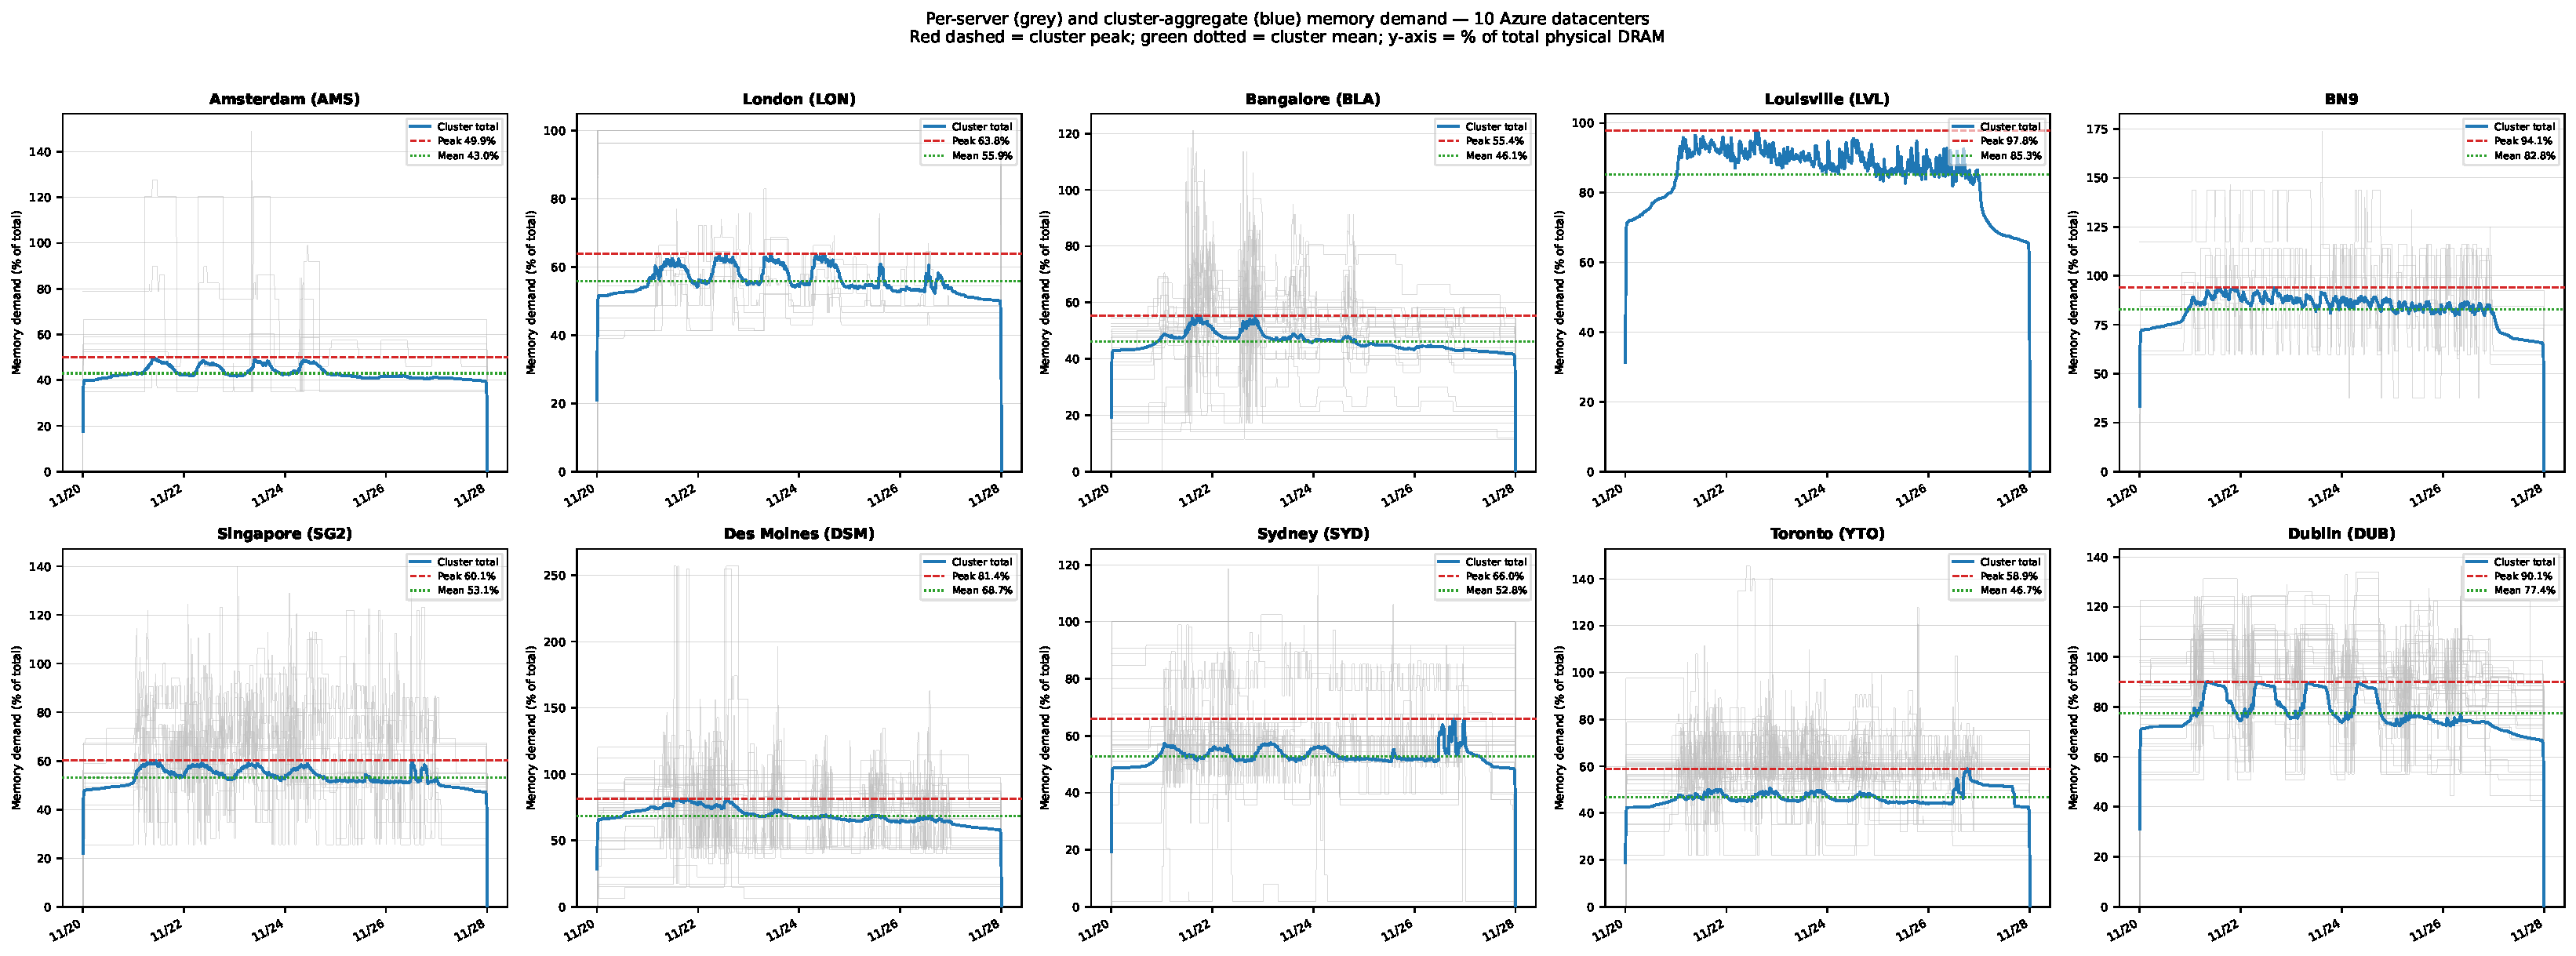
\includegraphics[width=\textwidth]{figs/demand_overview.pdf}
    \caption{%
        Per-server (grey) and cluster-aggregate (blue) memory demand across
        ten Azure datacenters.  Red dashed: cluster peak.  Green dotted:
        cluster mean.  $y$-axis: demand as a percentage of total physical
        DRAM installed in the cluster.  Traces span $\approx$14 days at
        5-minute resolution.
    }
    \label{fig:demand_overview}
\end{figure}

\subsubsection*{Diurnal Patterns}

Figure~\ref{fig:demand_diurnal} overlays all individual days (grey) together
with the mean (blue) and $\pm$1-standard-deviation band.  The diurnal pattern
is highly consistent across days, with low inter-day variance at off-peak
hours and higher variance during the busy period.  This regularity is
precisely what an RL agent can exploit: by learning the expected future
demand trajectory from the current time-of-day and recent history, it can
make allocation decisions that leave MPD headroom during predicted ramp-ups.

\begin{figure}[H]
    \centering
    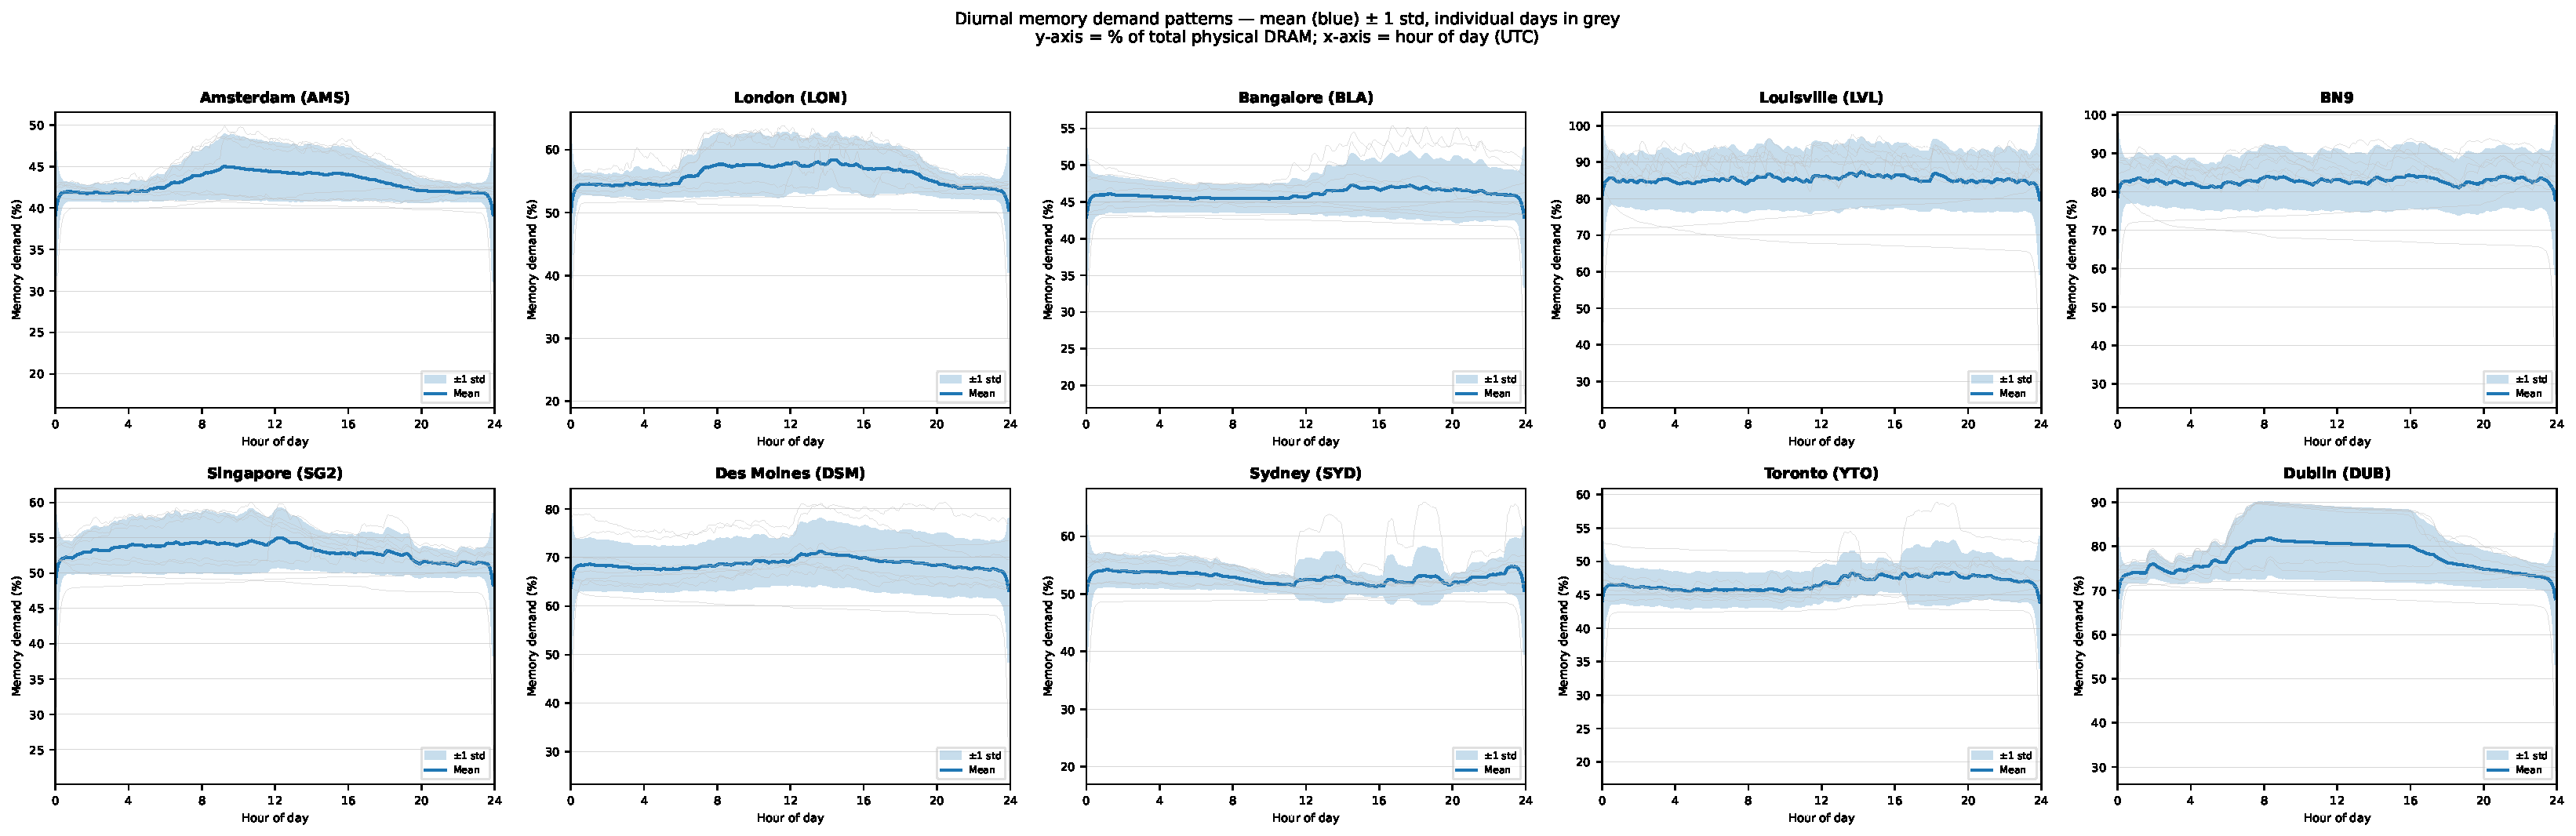
\includegraphics[width=\textwidth]{figs/demand_diurnal.pdf}
    \caption{%
        Diurnal memory demand profile for each datacenter.  Blue line: daily
        mean.  Blue band: $\pm$1 standard deviation.  Grey lines: individual
        days.  $x$-axis: hour of day (UTC).
    }
    \label{fig:demand_diurnal}
\end{figure}

\subsubsection*{Peak-to-Mean Ratio Across Datacenters}

Figure~\ref{fig:peak_to_mean} summarises the peak-to-mean ratio and the
absolute peak and mean demand levels for each datacenter.  A ratio of 1.5,
for example, means the cluster needs $50\%$ more CXL memory than its average
demand to handle its worst moment.  Pooling across servers within a site
reduces the \emph{effective} ratio by multiplexing uncorrelated per-server
peaks.

\begin{figure}[H]
    \centering
    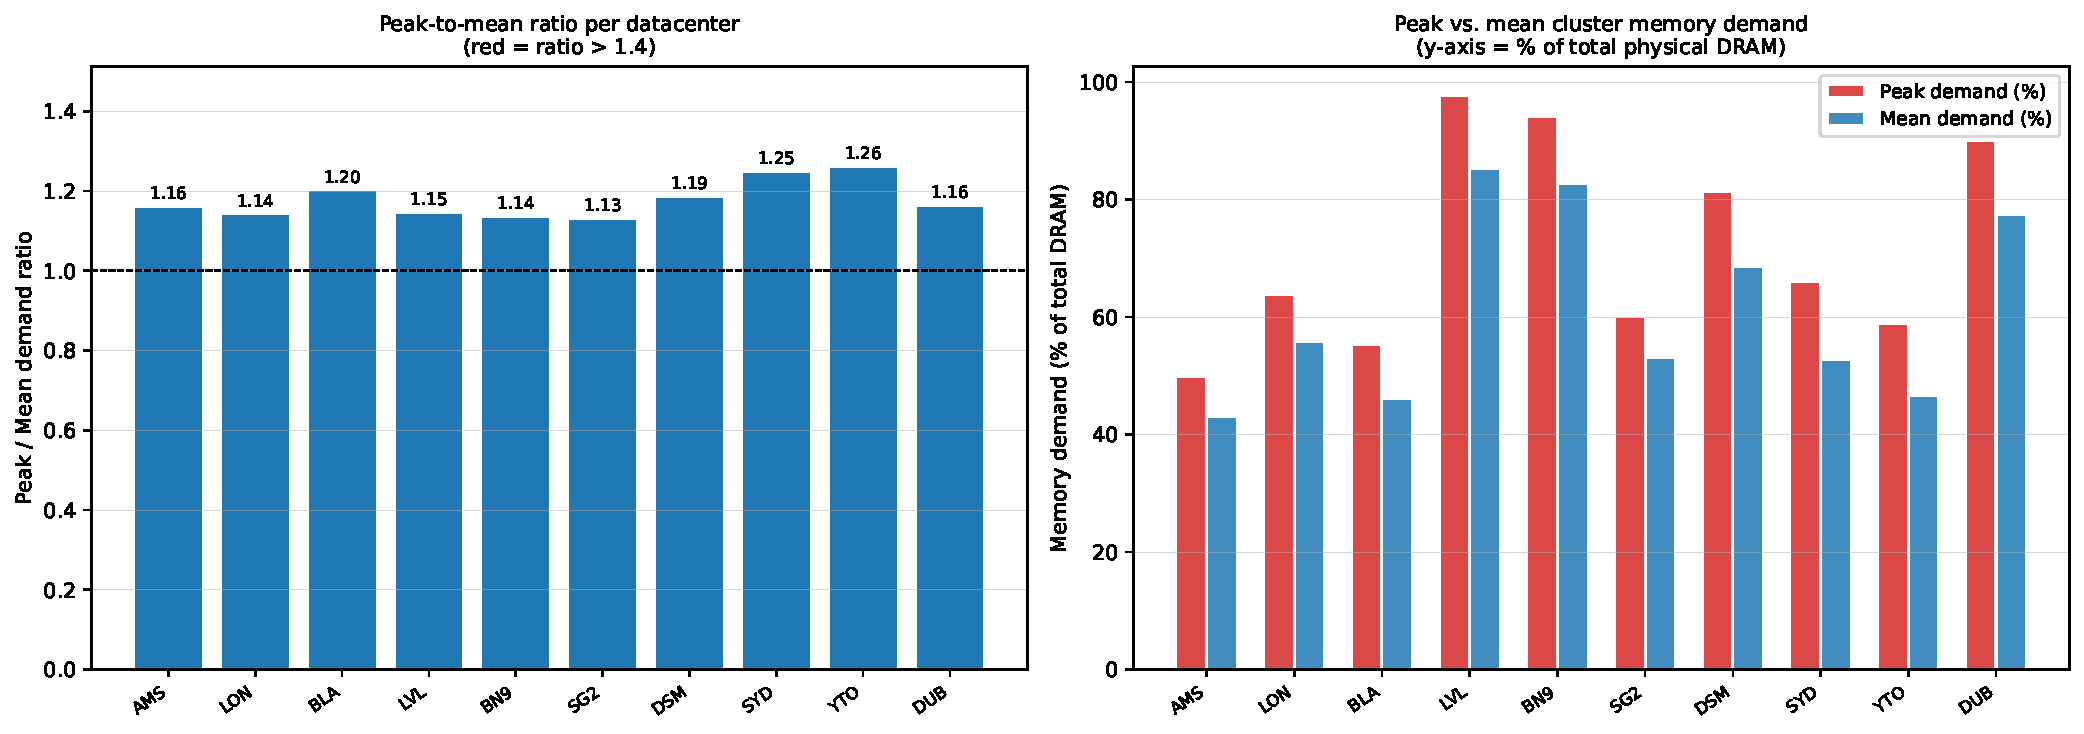
\includegraphics[width=\textwidth]{figs/peak_to_mean.pdf}
    \caption{%
        Left: peak-to-mean demand ratio per datacenter (red bars $> 1.4$).
        Right: absolute peak and mean demand as a fraction of total physical
        DRAM.  The gap between peak and mean (left panel) is the capacity that
        pooling recovers.
    }
    \label{fig:peak_to_mean}
\end{figure}

% ----------------------------------------------------------------------
\subsection{Assuming RL is \emph{Not} the Solution: Baseline Comparisons}
\label{sec:baselines}
% ----------------------------------------------------------------------

Before committing to an RL approach we evaluate two analytical baselines---a
practical heuristic and an exact offline optimum---to bound the space of
achievable pooling savings.

\subsubsection*{Greedy Baseline}

The greedy policy allocates each new VM's CXL memory from whichever
accessible MPD currently has the \emph{lowest} total load, splitting the
allocation evenly across tied MPDs when necessary.  No migration is ever
performed: once memory is allocated to an MPD it stays there until the VM
terminates.

Algorithm~\ref{alg:greedy} gives the per-VM allocation step.

\begin{algorithm}[H]
\SetAlgoLined
\KwIn{Request $x$ GB; list of accessible MPDs $\mathcal{N}$;
      current load vector $\mathbf{c} \in \mathbb{R}^m$}
\KwOut{Allocation vector $\mathbf{a}$}
$\mathbf{a} \leftarrow \mathbf{0}$\;
\While{$x > 0$}{
    $j^* \leftarrow \arg\min_{j \in \mathcal{N}} c_j$
    \quad (min-load MPD)\;
    $S \leftarrow \{j \in \mathcal{N} : c_j = c_{j^*}\}$
    \quad (all tied MPDs)\;
    $j' \leftarrow \arg\min_{j \in \mathcal{N},\; c_j > c_{j^*}} c_j$
    \quad (next-level MPD, or $\infty$)\;
    $\delta \leftarrow \min\!\left(x,\; |S|\cdot(c_{j'} - c_{j^*})\right)$\;
    \ForEach{$j \in S$}{
        $a_j \leftarrow a_j + \delta / |S|$\;
        $c_j \leftarrow c_j + \delta / |S|$\;
    }
    $x \leftarrow x - \delta$\;
}
\Return $\mathbf{a}$\;
\caption{Greedy allocation for a single VM arrival.}
\label{alg:greedy}
\end{algorithm}

The corresponding Python implementation in the notebook is:

\begin{lstlisting}[caption={Python implementation of greedy allocation.}]
def greedy_alloc(cxl_mem, mhd_list, cur_cxl_mem_vec):
    alloc_arr = np.zeros((len(cur_cxl_mem_vec),))
    cur_cxl_mem_vec = np.maximum(cur_cxl_mem_vec, np.zeros(...))
    while cxl_mem > 0:
        min_mhd = min(mhd_list, key=lambda j: cur_cxl_mem_vec[j])
        # ... fill to next level, split across tied MPDs ...
    return alloc_arr
\end{lstlisting}

\subsubsection*{Optimal Baseline}

The optimal policy has access to future VM arrival times and is allowed to
\emph{migrate} already-allocated memory between MPDs at any time.  This is
clearly impractical at runtime but provides an upper bound on pooling savings.

At each tick, the optimal allocation minimises the peak per-MPD load subject
to adjacency constraints:
\begin{equation}
\begin{aligned}
\min_{\mathbf{X}} \quad & \max_{j \in [m]} \sum_{i=1}^{n} X_{ij} \\
\text{s.t.} \quad & \sum_{j=1}^{m} X_{ij} = b_i \quad \forall i, \\
                  & X_{ij} \ge 0, \\
                  & X_{ij} = 0 \text{ if } M_{ij} = 0,
\end{aligned}
\label{eq:opt}
\end{equation}
where $b_i$ is the total CXL demand of server $i$ at the current tick.
This is a minimax flow problem and is solved exactly via a
\textbf{binary search + max-flow} (Dinic's algorithm) decomposition in
$O(T \cdot n \cdot m \cdot (n + m)^{0.5})$ time:

\begin{lstlisting}[caption={Optimal allocation via binary search on peak load.}]
def find_optimal(node_cxl_arr, M):
    # Binary search over feasible peak cap `t`:
    #   feasible(t) iff max-flow from src->hosts->MPDs->sink >= total demand
    #   (each host->MPD edge has capacity inf; each MPD->sink has capacity t)
    lo, hi = lower_bound(node_cxl_arr, M), sum(node_cxl_arr)
    for _ in range(30):          # 30 iterations -> 1e-9 relative precision
        mid = 0.5 * (lo + hi)
        if feasible(mid): hi = mid
        else:             lo = mid
    return hi                    # optimal peak per-MHD
\end{lstlisting}

The feasibility check for a given capacity $t$ is a standard bipartite
max-flow: a source is connected to each server node with edge capacity
$b_i$; server nodes are connected to their reachable MPDs with infinite
capacity; each MPD is connected to a sink with capacity $t$.
The allocation is feasible iff the max-flow equals $\sum_i b_i$.

\subsubsection*{PID Controller Baseline}

A PID (Proportional--Integral--Derivative) controller is a classical
feedback mechanism that adjusts an output signal to drive a measured
\emph{error} toward zero.  We adapt it here as a load-balancing baseline:
the controller tracks how far each MPD's load deviates from the
\emph{cluster average}, and biases new VM allocations toward under-loaded
MPDs proportionally to that deviation.

\paragraph{Error signal.}
Let $\bar{c}(t) = \frac{1}{m}\sum_j c_j(t)$ be the mean MPD load at tick
$t$.  For each MPD $j$, define the load error:
\[
    e_j(t) = \bar{c}(t) - c_j(t).
\]
A positive error means MPD $j$ is \emph{below} average and should receive
more allocation; a negative error means it is overloaded and should receive
less.

\paragraph{PID signal.}
The controller accumulates three terms per MPD:
\[
    u_j(t) = K_P\, e_j(t)
           + K_I \sum_{\tau=0}^{t} e_j(\tau)
           + K_D \bigl(e_j(t) - e_j(t-1)\bigr),
\]
with gains $K_P, K_I, K_D \ge 0$.

\paragraph{Allocation rule.}
When a VM with demand $x$ arrives on server $i$, the PID score for each
accessible MPD $j \in \mathcal{N}(i)$ is $u_j(t)$.  The allocation is
split \emph{in proportion to the softmax of the scores}, so that heavily
under-loaded MPDs receive a larger share:
\[
    w_j = \frac{\exp\!\bigl(u_j(t) / \tau\bigr)}
               {\sum_{k \in \mathcal{N}(i)} \exp\!\bigl(u_k(t) / \tau\bigr)},
    \qquad
    a_j = x \cdot w_j,
\]
where $\tau > 0$ is a temperature that controls how sharply the allocation
concentrates on the best MPD ($\tau \to 0$ recovers the greedy argmin;
$\tau \to \infty$ gives a uniform split).

Algorithm~\ref{alg:pid} summarises the per-VM step.

\begin{algorithm}[H]
\SetAlgoLined
\KwIn{Request $x$ GB; accessible MPDs $\mathcal{N}$;
      load vector $\mathbf{c}$; PID state $(\mathbf{e}_{\text{prev}}, \boldsymbol{\sigma})$;
      gains $K_P, K_I, K_D$; temperature $\tau$}
\KwOut{Allocation $\mathbf{a}$}
$\bar{c} \leftarrow \frac{1}{|\mathcal{N}|}\sum_{j \in \mathcal{N}} c_j$\;
\ForEach{$j \in \mathcal{N}$}{
    $e_j \leftarrow \bar{c} - c_j$\;
    $\sigma_j \leftarrow \sigma_j + e_j$ \quad (integral)\;
    $u_j \leftarrow K_P e_j + K_I \sigma_j + K_D(e_j - e_{j,\text{prev}})$\;
}
$w_j \leftarrow \mathrm{softmax}(\mathbf{u} / \tau)_j$ for each $j \in \mathcal{N}$\;
$\mathbf{a} \leftarrow x \cdot \mathbf{w}$\;
$\mathbf{e}_{\text{prev}} \leftarrow \mathbf{e}$\;
\Return $\mathbf{a}$\;
\caption{PID allocation for a single VM arrival.}
\label{alg:pid}
\end{algorithm}

\paragraph{Role of the baseline.}
The PID controller is strictly reactive: it acts on the \emph{current}
imbalance but has no model of future demand.  It captures more signal than
the greedy policy (it uses both the integral of past imbalances and the
rate of change), making it a stronger rule-based baseline.  The gap between
PID and the RL policy therefore isolates the value of \emph{learned
anticipation} of future demand over a well-tuned feedback rule.
Default gains used in experiments: $K_P = 1.0$, $K_I = 0.01$,
$K_D = 0.1$, $\tau = 1.0$.

\subsubsection*{Simulation Results}

Table~\ref{tab:greedy_vs_opt} summarises pooling savings for the
\texttt{AG16x6\_expander\_quads} topology (16 hosts, 6 MPDs, regular
expander with $r = 5$, 50 random node-to-pod mappings):

\begin{table}[H]
\centering
\small
\begin{tabular}{lcccc}
\toprule
\textbf{Policy} & \textbf{Avg savings} & \textbf{Min} & \textbf{Max} & \textbf{Std} \\
\midrule
Greedy (no migration)          & \red{TODO} & \red{TODO} & \red{TODO} & \red{TODO} \\
PID controller ($K_P{=}1, K_I{=}0.01, K_D{=}0.1$) & \red{TODO} & \red{TODO} & \red{TODO} & \red{TODO} \\
Static Optimal (4-hr window)   & 94.5\%     & ---        & ---        & ---        \\
Static Optimal (8-hr window)   & 92.3\%     & ---        & ---        & ---        \\
Optimal (full migration)       & 88.3\%     & ---        & ---        & ---        \\
\bottomrule
\end{tabular}
\caption{Pooling savings for regular Octopus topology (X=5, N=4, $\lambda=1$):
16 hosts, 20 MPDs, 50\% VM memory in CXL\@.
Results from Yuhong's slides (Feb 2026).
Greedy simulation pending on AMS20 trace; \red{TODO: fill once run completes}.}
\label{tab:greedy_vs_opt}
\end{table}

Table~\ref{tab:random96} shows greedy savings for the \texttt{random\_L96}
topology (96 hosts, 8 MHDs per host, $N=4$ hosts per pod) on the AMS20 trace
over 50 random pod assignments:

\begin{table}[H]
\centering
\small
\begin{tabular}{lccccc}
\toprule
\textbf{Topology} & \textbf{Hosts} & \textbf{MHDs} & \textbf{Avg savings} & \textbf{Std} \\
\midrule
\texttt{random\_L96\_X8\_N4} & 96 & 8 & 26.3\% & 0.0 \\
\bottomrule
\end{tabular}
\caption{Greedy pooling savings on the AMS20 trace (50 random pod mappings).
Savings metric: $1 - \text{peak CXL}/\text{total DRAM}$.}
\label{tab:random96}
\end{table}

\subsubsection*{Fully-Connected vs.\ Sparse Octopus Topology}

Figure~\ref{fig:fc_vs_octopus} compares the pooling savings achieved by a
fully-connected topology (every host can reach every MPD) against a regular
Octopus topology ($N = 4$ hosts per MPD, degree 8) under the greedy
allocation policy, sweeping pod size and CXL fraction on the LON23 trace.

Three CXL fractions are shown: 10\%, 30\%, and 50\% of each VM's memory
placed on CXL\@.  Two consistent trends emerge:

\begin{itemize}
    \item \textbf{Savings increase with CXL fraction.}  At 10\% CXL the
          pooling benefit is inherently small (only a thin slice of memory
          participates); savings sit near 90--92\%.  At 50\% CXL the savings
          drop to 50--62\%, reflecting the substantially larger CXL footprint
          that now demands real load balancing.

    \item \textbf{Fully-connected consistently outperforms sparse Octopus.}
          The gap is negligible at 10\% CXL ($< 1$ pp) but widens to
          3--7 percentage points at 50\% CXL\@.  This confirms the intuition
          that sparse connectivity restricts the allocation algorithm's
          ability to spread demand evenly.
\end{itemize}

\begin{figure}[H]
    \centering
    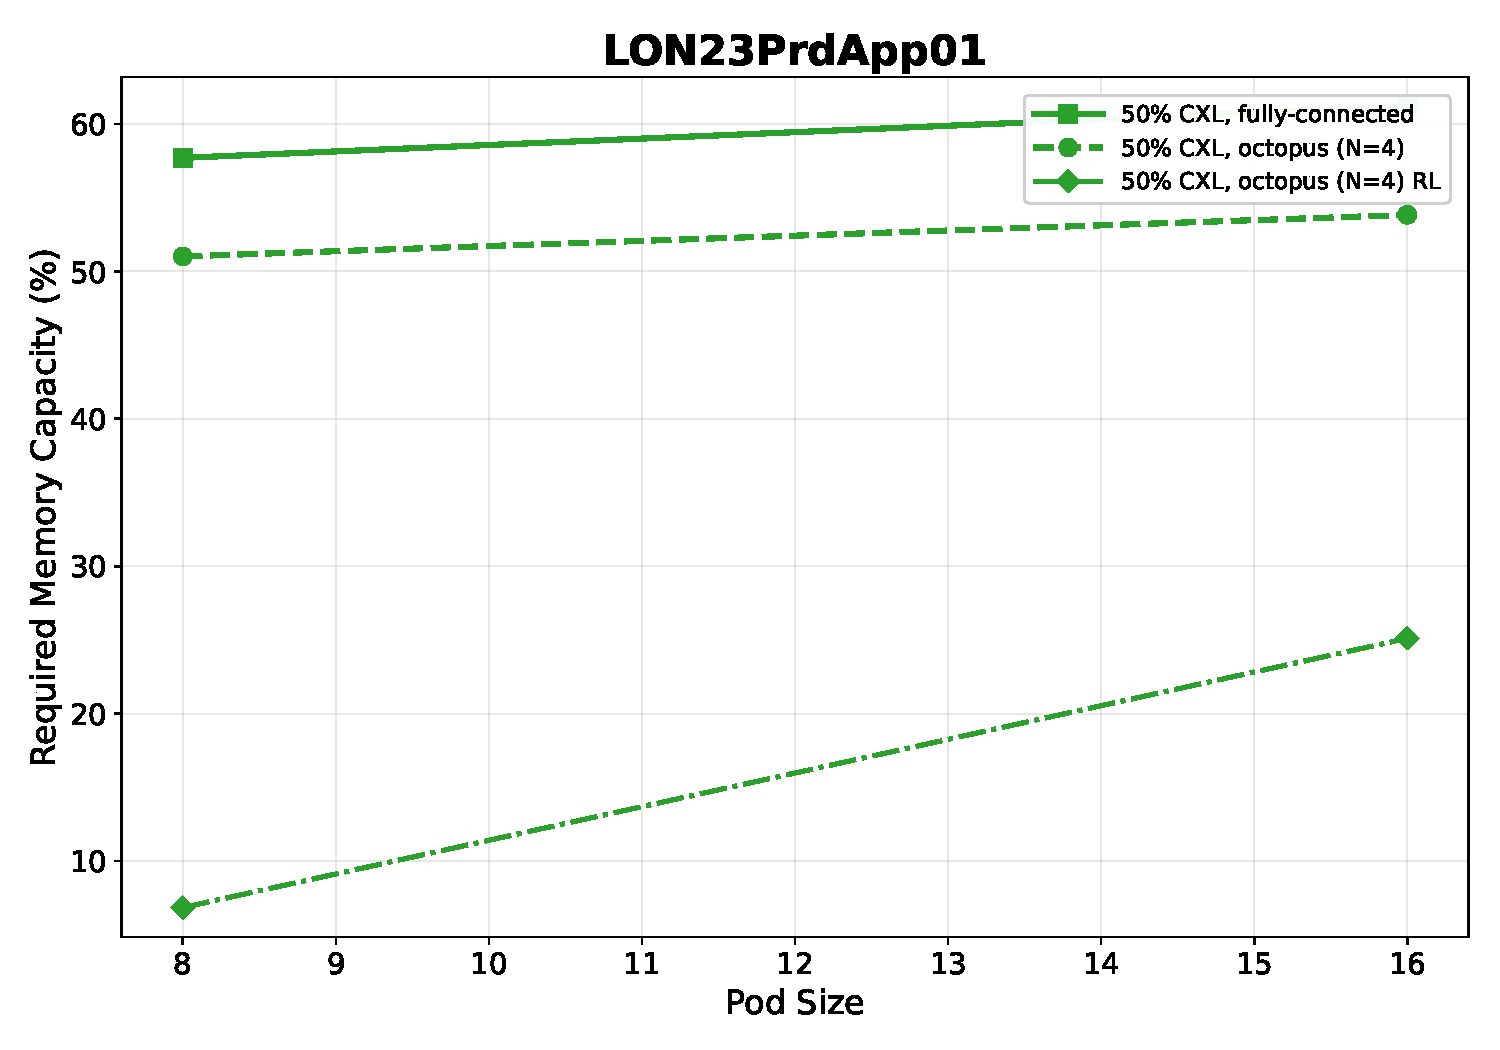
\includegraphics[width=0.85\textwidth]{figs/fc_vs_octopus.pdf}
    \caption{%
        Pooling savings (\%) vs.\ pod size for three CXL fractions.
        Solid lines: fully-connected topology.  Dashed lines: regular
        Octopus ($N{=}4$, greedy allocation).  LON23 trace, 5 random
        pod mappings per point.  Higher values indicate less CXL capacity
        required relative to total pod DRAM\@.
    }
    \label{fig:fc_vs_octopus}
\end{figure}

Figure~\ref{fig:3panel} separates the same data into per-CXL-fraction
panels, making the pod-size scaling easier to read.  At 50\% CXL the
fully-connected topology gains roughly 7~pp in savings between pod size 4
and 16, while the Octopus topology gains only 5~pp---indicating that larger
pods amplify the advantage of richer connectivity.

\begin{figure}[H]
    \centering
    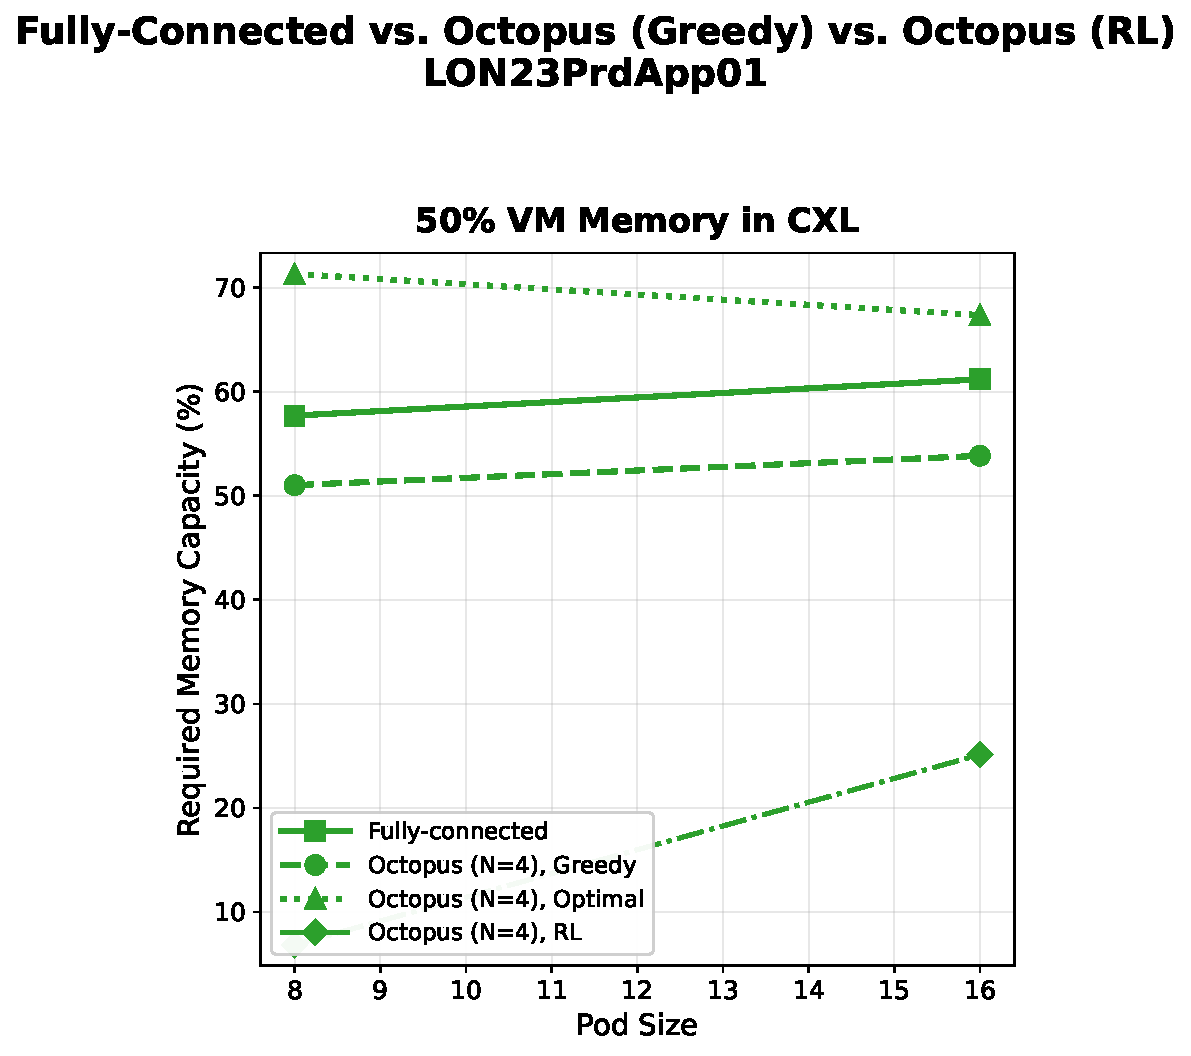
\includegraphics[width=\textwidth]{figs/3panel_by_cxl.pdf}
    \caption{%
        Per-CXL-fraction panels: fully-connected (solid, squares) vs.\
        Octopus greedy (dashed, circles).  LON23 trace, 5 random pod
        mappings.
    }
    \label{fig:3panel}
\end{figure}

\subsubsection*{MHD Load Balancing: Greedy vs.\ RL Time Series}

To understand \emph{how} the allocation policies distribute load across
MPDs, Figures~\ref{fig:ts_greedy} and~\ref{fig:ts_rl} plot per-MHD memory
usage over the full $\approx$8-day trace window for the top-12 most loaded
MHDs (Octopus topology, 50\% CXL, pod size 16).

\paragraph{Greedy (Figure~\ref{fig:ts_greedy}).}
The greedy policy achieves a reasonably balanced load distribution: the
most loaded MHD peaks at $\approx$104\,k\,GB and the least loaded at
$\approx$46\,k\,GB, a ratio of roughly 2.3$\times$.  The traces show
correlated diurnal swings across MHDs, with load tracking the cluster-wide
demand cycle.  The moderate spread confirms that greedy's myopic
least-loaded rule does a passable---though not optimal---job of spreading
demand.

\begin{figure}[H]
    \centering
    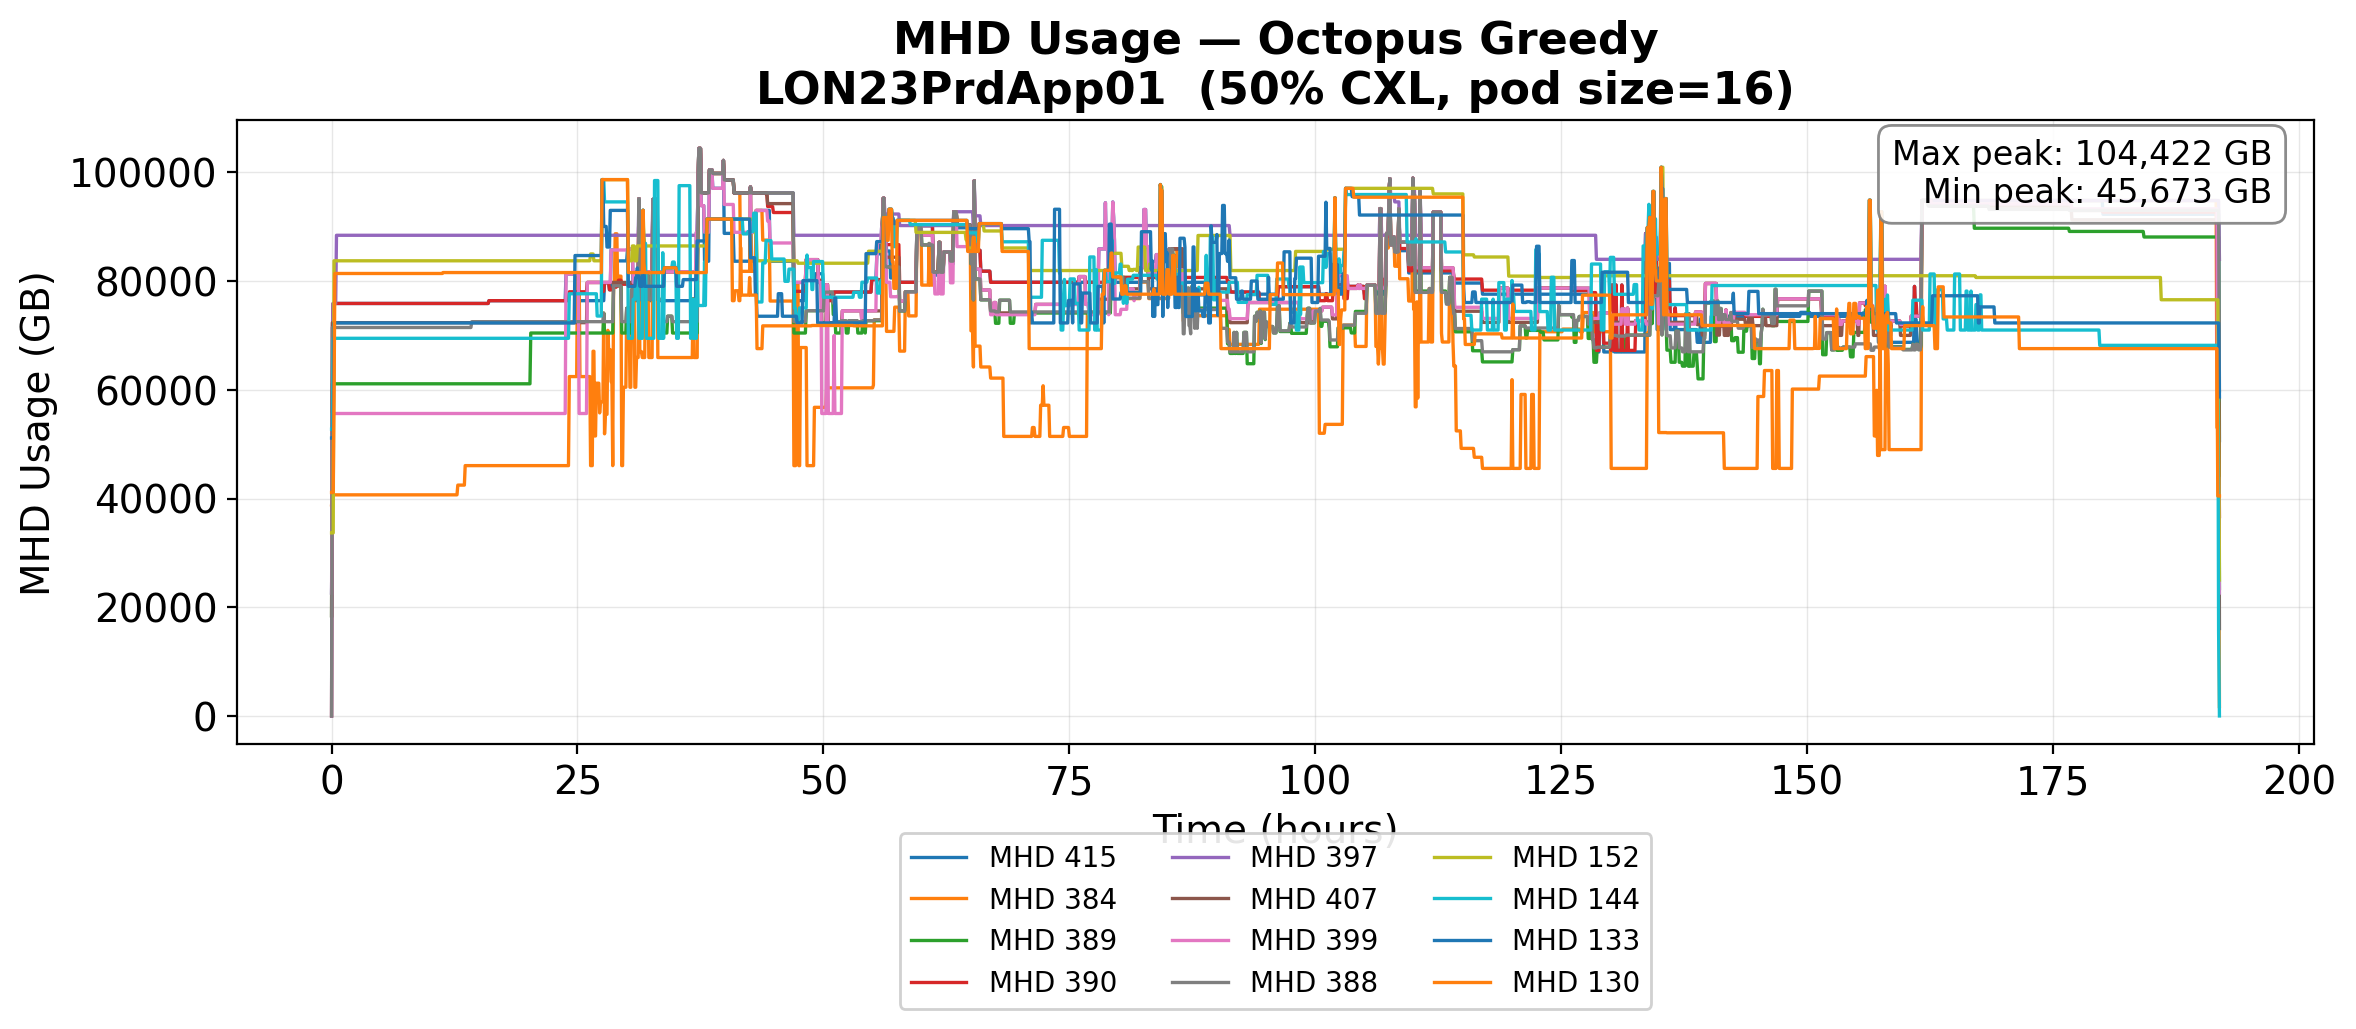
\includegraphics[width=\textwidth]{figs/mhd_timeseries_greedy.png}
    \caption{%
        Per-MHD memory usage over time under the greedy allocation policy.
        Octopus topology ($N{=}4$), 50\% CXL, pod size 16, LON23 trace.
        Top-12 MHDs by peak load are shown.
    }
    \label{fig:ts_greedy}
\end{figure}

\paragraph{RL --- SAC, 1M timesteps (Figure~\ref{fig:ts_rl}).}
The RL agent (SAC, 1\,M training timesteps, fast hyperparameters) exhibits
a qualitatively different---and worse---load profile.  The most loaded MHD
peaks at $\approx$183\,k\,GB while the least loaded reaches only
$\approx$9\,k\,GB, a ratio exceeding 20$\times$.  The agent has learned to
concentrate load on a handful of MHDs, leaving others nearly idle.

\begin{figure}[H]
    \centering
    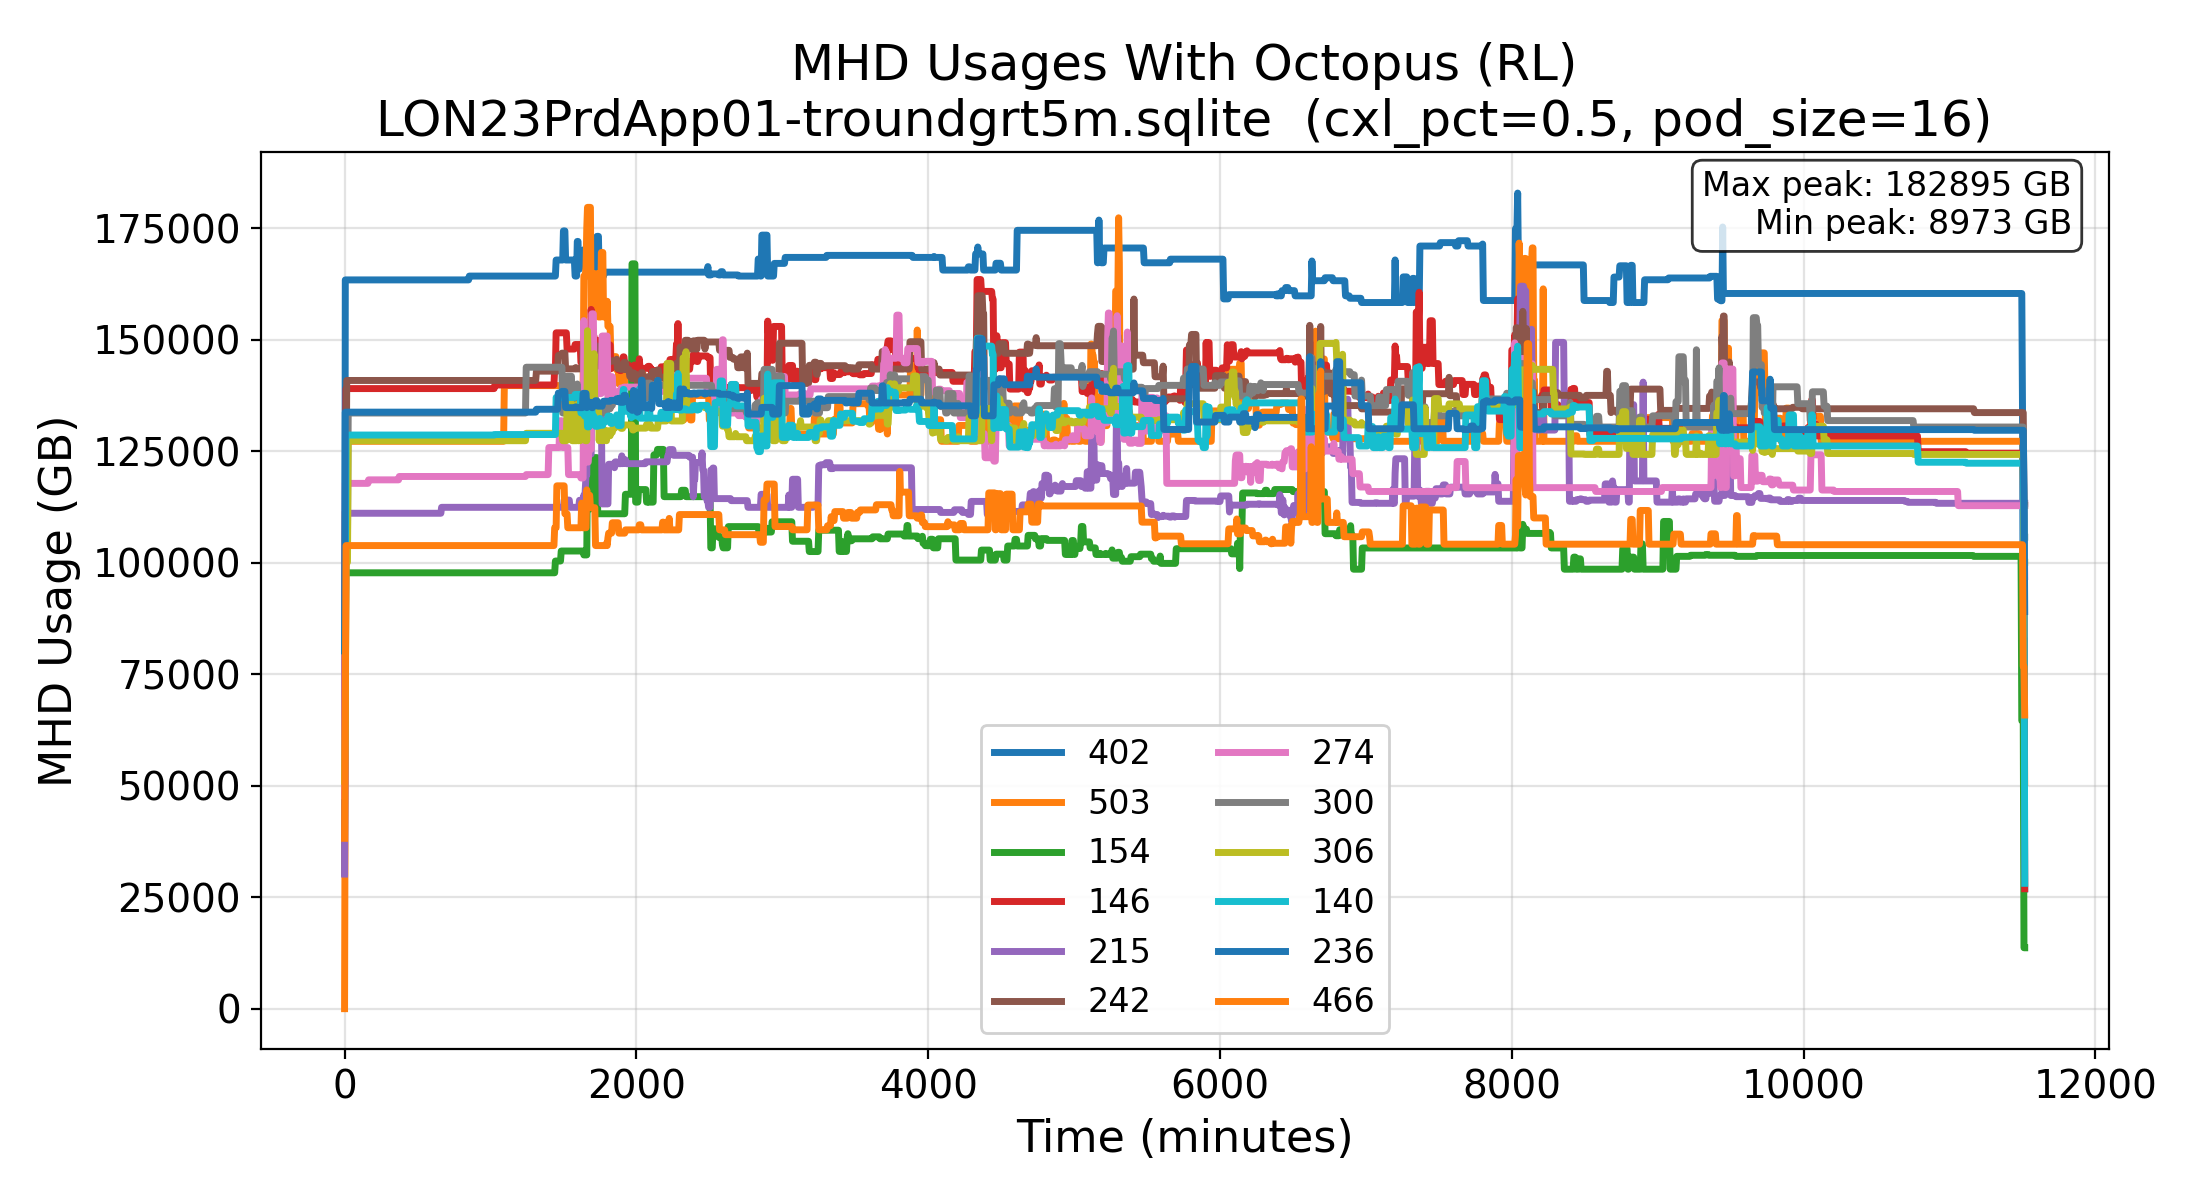
\includegraphics[width=\textwidth]{figs/mhd_timeseries_rl.png}
    \caption{%
        Per-MHD memory usage over time under the RL (SAC) allocation policy.
        Same topology and trace as Figure~\ref{fig:ts_greedy}.  The
        pronounced load imbalance---max/min ratio $> 20\times$---shows
        the agent has failed to learn balanced allocation.
    }
    \label{fig:ts_rl}
\end{figure}

\subsubsection*{Preliminary RL Assessment}

The current RL policy underperforms the greedy baseline on every metric.
The root cause is visible in the time-series comparison: the agent has not
learned to balance load across MHDs.  Several factors likely contribute:

\begin{enumerate}
    \item \textbf{Reward signal.}  The per-step reward penalises increases
          in the global peak load ($-\Delta \max_j c_j$), but this signal
          is sparse: only the single worst MHD produces a non-zero gradient,
          giving the agent no incentive to balance the remaining devices.
          Adding a variance-based shaping term
          ($-\lambda \operatorname{Var}(\mathbf{c})$) would provide a
          denser learning signal.

    \item \textbf{Insufficient training.}  1\,M timesteps with
          \texttt{train\_freq=16} yields only $\sim$62\,k gradient updates,
          which may be too few for the agent to learn the temporal structure
          of a multi-day trace.

    \item \textbf{Train/eval topology mismatch.}  The training environment
          uses a fixed small topology (16 hosts); the evaluation sweeps
          multiple random pod mappings.  Generalisation across pod
          assignments is non-trivial and may require domain randomisation
          during training.
\end{enumerate}

These findings motivate the reward-shaping and extended-training experiments
described in Section~\ref{sec:next_steps}.

\subsubsection*{Effect of Link Failures}

To stress-test robustness, edges are randomly removed from the topology
(modelling CXL link failures or maintenance).  Table~\ref{tab:failures} shows
how greedy savings degrade as a fraction of links are removed from the
\texttt{AG16x6\_expander\_quads} topology:

\begin{table}[H]
\centering
\small
\begin{tabular}{lccccc}
\toprule
\textbf{Failure ratio} & \textbf{Avg savings} & \textbf{Min} & \textbf{Max} & \textbf{Std} \\
\midrule
0.01 & 24.65\% & 17.29\% & 29.60\% & 2.88\% \\
0.02 & 23.59\% & 15.56\% & 29.28\% & 2.87\% \\
0.03 & 22.87\% & 11.57\% & 28.76\% & 3.14\% \\
0.04 & 22.07\% & 11.46\% & 28.59\% & 3.00\% \\
0.05 & 21.25\% & 11.46\% & 28.58\% & 3.27\% \\
0.10 & 14.80\% & $-$4.08\% & 24.94\% & 6.03\% \\
\bottomrule
\end{tabular}
\caption{Greedy pooling savings as a function of random link-failure rate
(50 iterations each).  Savings degrade gracefully up to $\sim$5\% failures,
then drop sharply at 10\% (some pods become infeasible, yielding negative
savings).}
\label{tab:failures}
\end{table}

The greedy-to-optimal gap (Table~\ref{tab:greedy_vs_opt}) motivates a
learned policy: a policy with \emph{lookahead} about future demand should
be able to close part of this gap without requiring full migration.

% ======================================================================
\section{Building the RL Policy and Environment}
% ======================================================================

The RL environment wraps the Octopus memory pooling simulator.  Each VM
arrival is a decision point; the agent observes the current system state,
selects an allocation action, and receives a reward reflecting the quality of
that allocation.

% ----------------------------------------------------------------------
\subsection{States}
\label{sec:states}
% ----------------------------------------------------------------------

The state at decision time (VM arrival on host $i$) must encode enough
information for the agent to reason about future MPD load.

\subsubsection*{Current Implementation (v0)}

The initial prototype uses a compact observation vector of size
$2 \cdot d_{\max} + 4$, where $d_{\max}$ is the maximum host degree in the
topology.  Table~\ref{tab:states_v0} lists every component.

\begin{table}[H]
\centering
\small
\renewcommand{\arraystretch}{1.3}
\begin{tabular}{llcl}
\toprule
\textbf{Slice} & \textbf{Signal} & \textbf{Size} & \textbf{Encoding} \\
\midrule
$[0 \;:\; d_{\max})$
  & Accessible MPD loads
  & $d_{\max}$
  & $c_j / D_{\text{pod}}$, zero-padded for $j \notin \mathcal{N}(i)$ \\
$[d_{\max} \;:\; 2 d_{\max})$
  & Accessibility mask
  & $d_{\max}$
  & $1$ if MPD slot is valid, $0$ otherwise \\
$[2 d_{\max}]$
  & VM memory request
  & 1
  & $x / D_{\text{pod}}$ \\
$[2 d_{\max}{+}1]$
  & Global peak MPD load
  & 1
  & $\max_j c_j / D_{\text{pod}}$ \\
$[2 d_{\max}{+}2]$
  & Hour-of-day (sin)
  & 1
  & $\sin(2\pi\, h / 24)$ \\
$[2 d_{\max}{+}3]$
  & Hour-of-day (cos)
  & 1
  & $\cos(2\pi\, h / 24)$ \\
\bottomrule
\end{tabular}
\caption{v0 observation vector ($\texttt{OctopusMemPoolEnv.\_get\_obs}$).
All load values are normalised by total pod DRAM $D_{\text{pod}}$.
For the \texttt{AG16x6} topology ($d_{\max} = 8$), the observation
has 20 dimensions.}
\label{tab:states_v0}
\end{table}

\paragraph{Limitations.}
This minimal state is sufficient for initial training but lacks several
signals that could improve policy quality:

\begin{itemize}
    \item \textbf{No temporal context.}  The agent sees a single snapshot
          of MPD loads with no velocity or trend information.  It cannot
          distinguish a load that is ramping up from one that is declining,
          limiting its ability to anticipate future peaks.
    \item \textbf{No per-host memory pressure.}  The observation encodes
          only the \emph{accessible} MPD loads for the arriving VM's host,
          not the overall utilisation of each server.  A host nearing
          physical DRAM capacity will generate more CXL spill, but the agent
          has no signal to anticipate this.
    \item \textbf{No VM lifetime or workload profile.}  All VMs look
          identical except for their memory size.  A short-lived VM and a
          week-long VM receive the same treatment, even though the long-lived
          VM has a far larger impact on future MPD headroom.
    \item \textbf{No SLO violation feedback.}  The agent receives no
          explicit signal about past over-capacity events, making it
          difficult to learn conservative allocation strategies.
\end{itemize}

\subsubsection*{Proposed State Space (v1)}

To address these gaps, the target state space is organised into three
categories: Resource Health, Workload, and Topology.
For signals with temporal context, we encode history as current value plus
delta terms rather than raw window concatenation, making velocity signals
explicit and reducing the learning burden on the agent.
Table~\ref{tab:states} defines the full proposed state space.

\begin{landscape}
\begin{table}[H]
\centering
\renewcommand{\arraystretch}{1.6}
\setlength{\tabcolsep}{6pt}
\begin{tabularx}{\linewidth}{|c|l|X|l|l|X|}
\hline
\textbf{\#} & \textbf{Category} & \textbf{Signal} & \textbf{Temporal Treatment} & \textbf{Name} & \textbf{Encoding} \\
\hline
1 & Resource Health & Per-MPD capacity utilization (\% full)
  & 3 windows, 1-hr & \texttt{mpd\_cap}
  & $[v_t,\ \Delta_{1h},\ \Delta_{2h}]\ \times\ N_\text{MPD}$ \\
\hline
2 & Resource Health & Per-MPD bandwidth utilization (\% full)
  & Current snapshot & \texttt{mpd\_bw}
  & $[v_t]\ \times\ N_\text{MPD}$ \\
\hline
3 & Resource Health & Server memory pressure (\% RAM utilized)
  & 3 windows, 1-hr & \texttt{mem\_press}
  & $[v_t,\ \Delta_{1h},\ \Delta_{2h}]\ \times\ N_\text{servers}$ \\
\hline
4 & Resource Health & Recent SLO violations (over-capacity events)
  & 24-hr historical summary & \texttt{slo\_vio}
  & Scalar (\% allocations causing MPD overflow) \\
\hline
5 & Workload & Incoming VM size (requested memory)
  & Current snapshot & \texttt{vm\_size}
  & Scalar (GB) \\
\hline
6 & Workload & Predicted VM lifetime
  & Current snapshot & \texttt{vm\_lifetime}
  & Scalar (hours) \\
\hline
7 & Workload & Customer peak-to-average ratio
  & 24-hr historical summary & \texttt{pta}
  & $\max(\text{usage}_{24h})\ /\ \text{mean}(\text{usage}_{24h})$ \\
\hline
8 & Workload & Predicted future memory (growth rate)
  & Current snapshot & \texttt{future\_mem}
  & Scalar (GB/hr) \\
\hline
9 & Topology & Server-to-MPD connectivity mask
  & Static & \texttt{conn\_mask}
  & Binary vector $\in \{0,1\}^{N_\text{MPD}}$ \\
\hline
\end{tabularx}
\caption{State space for the single central RL controller. $v_t$ denotes
the current value; $\Delta_{1h}$, $\Delta_{2h}$ denote deltas from 1 and
2 hours prior respectively. \texttt{conn\_mask} is a static topology signal
used as a validity mask over the action space.}
\label{tab:states}
\end{table}
\end{landscape}

% ----------------------------------------------------------------------
\subsection{Actions}
\label{sec:actions}
% ----------------------------------------------------------------------

The action $a_t$ specifies how to distribute the VM's CXL request $x$ across
accessible MPDs. The agent outputs a continuous weight vector over the $k$
MPDs reachable from the arriving VM's server:

\begin{equation}
    \mathbf{a} = [w_1, w_2, \ldots, w_k] \in \mathbb{R}^k
    \label{eq:action}
\end{equation}

subject to the following constraints:

\begin{align}
    w_i &\geq 0 \quad \forall\, i \label{eq:nonneg} \\
    \sum_{i=1}^{k} w_i &= 1 \label{eq:sum} \\
    w_i &= 0 \quad \text{if } \texttt{conn\_mask}_i = 0 \label{eq:mask}
\end{align}

The weight vector is translated into a physical allocation as follows:

\begin{equation}
    \text{GB allocated from MPD}_i = w_i \times \texttt{vm\_size}
    \label{eq:alloc}
\end{equation}

The connectivity mask (\texttt{conn\_mask}) is applied prior to the softmax
output layer, zeroing out unreachable MPDs. The softmax then normalises the
remaining weights to satisfy Equation~\ref{eq:sum}. Table~\ref{tab:actions}
summarises all agent actions and their abstraction level.

\begin{table}[H]
\centering
\renewcommand{\arraystretch}{1.6}
\setlength{\tabcolsep}{8pt}
\begin{tabularx}{\linewidth}{|c|X|l|X|}
\hline
\textbf{\#} & \textbf{Action} & \textbf{Type} & \textbf{Abstraction Level} \\
\hline
1 & Allocation split $\mathbf{a} = [w_1, \ldots, w_k]$ across connected MPDs
  & Continuous & High-level strategic $\rightarrow$ RL \\
\hline
2 & \texttt{flag\_migration(vm\_id)} --- flag a VM for migration
  & Binary & High-level strategic $\rightarrow$ RL \\
\hline
--- & Physical page placement & Mechanical & Low-level $\rightarrow$ system \\
\hline
--- & Address mapping updates & Mechanical & Low-level $\rightarrow$ system \\
\hline
\end{tabularx}
\caption{Action space for the single central RL controller. Actions 1 and 2
are high-level strategic decisions made by the RL agent. Physical page
placement and address mapping are handled mechanically by the system and are
transparent to the agent.}
\label{tab:actions}
\end{table}

% ----------------------------------------------------------------------
\subsection{Reward}
\label{sec:reward}
% ----------------------------------------------------------------------

The reward should incentivise \emph{balanced} MPD usage so that the eventual
peak load (and thus required CXL capacity) is minimised. We evaluate two
reward formulations. Option A serves as the simpler baseline; Option B
extends it with a delayed component to improve credit assignment over the
VM lifetime.

\subsubsection*{Option A: Fully Immediate, Smooth}

All components are evaluated at VM arrival time. The SLO violation penalty
is proportional and smooth, providing stable gradient signal for SAC.

\begin{equation}
    R = \alpha \cdot \left(1 - \frac{\max(\texttt{mpd\_cap})}{\texttt{mpd\_cap\_max}}\right)
      - \beta \cdot \texttt{slo\_vio}
      - \gamma \cdot \mathbb{1}[\texttt{flag\_migration}]
    \label{eq:reward_a}
\end{equation}

where $\alpha,\ \beta,\ \gamma > 0$ are weights reflecting objective priority,
with $\alpha < \beta$ to enforce SLO priority over utilization.

\subsubsection*{Option B: Immediate + Delayed}

Option B decomposes the reward into an immediate component at VM arrival
and a delayed component at VM termination, discounted by the VM lifetime $T$.
The immediate component provides smooth gradient signal; the delayed component
applies hard penalties for actual SLO violations and migrations over the
VM's lifetime.

\begin{equation}
    R_t = \underbrace{\alpha \cdot \left(1 - \frac{\max(\texttt{mpd\_cap})}{\texttt{mpd\_cap\_max}}\right)}_{\text{immediate at arrival}}
        + \underbrace{\lambda^{T} \left(- \beta \cdot \texttt{slo\_vio}_{T} - \delta \cdot \mathbb{1}[\text{migrated}]\right)}_{\text{delayed at termination}}
    \label{eq:reward_b}
\end{equation}

where $T$ is the VM lifetime in hours (known at arrival via \texttt{vm\_lifetime}),
$\lambda \in (0,1)$ is the discount factor, and $\beta > \delta$ ensures SLO
violations are penalised more heavily than migration.

\noindent\textbf{Note:} In both formulations, weights $\alpha$, $\beta$,
$\gamma$, $\delta$ are initially manually tuned and reflect the objective
priority ordering (utilization $\prec$ SLO $\prec$ migration). Future work
will explore online weight adaptation via multi-objective RL (MORL) to remove
the need for manual tuning, directly addressing a known limitation of
FleetIO~\cite{fleetio2025}.

% ----------------------------------------------------------------------
\subsection{Model}
\label{sec:model}
% ----------------------------------------------------------------------

Two RL algorithms are evaluated, plus a constrained variant:

\subsubsection*{Soft Actor-Critic (SAC)}

SAC~\cite{haarnoja2018sac} is an off-policy, maximum-entropy RL algorithm
for continuous action spaces.  It trains a stochastic policy $\pi_\phi$ by
jointly maximising expected reward and action entropy:
\[
    J(\pi) = \mathbb{E}\!\left[\sum_t \bigl(r_t + \alpha \mathcal{H}(\pi(\cdot \mid s_t))\bigr)\right],
\]
where $\alpha$ is a temperature parameter (learnable or fixed).  SAC is chosen
as the primary model because:
\begin{itemize}
    \item Our action space is continuous ($\mathbb{R}^m$) and SAC is
          sample-efficient in this regime.
    \item The entropy term prevents premature collapse to deterministic
          policies that over-specialise on training workloads.
    \item SAC has strong empirical performance on resource-management tasks
          (FleetIO uses a related off-policy approach).
\end{itemize}

\subsubsection*{Proximal Policy Optimisation (PPO)}

PPO~\cite{schulman2017ppo} is an on-policy algorithm that clips the policy
gradient update to prevent large policy shifts.  It serves as a fallback for
cases where SAC's replay buffer struggles with the temporal non-stationarity
of VM workloads (a known SAC weakness on highly correlated sequential data).

\subsubsection*{Locally Constrained Policy Optimisation (LCPO)}

Online RL in production systems faces \emph{catastrophic forgetting} (CF):
as the agent trains on new experiences, it overwrites knowledge acquired
from earlier workload regimes.  This is a concrete risk in our setting ---
diurnal demand cycles and workload shifts mean that the distribution of
VM arrivals changes continuously, and an agent that forgets morning-hour
patterns by the evening will make poor allocation decisions the next day.

LCPO~\cite{hamadanian2025lcpo} directly addresses CF in non-stationary,
context-driven environments.  Rather than relying on task labels (which
are unavailable in production) or brittle regularisation heuristics, LCPO
\emph{locally constrains} each policy-gradient update by anchoring the new
policy on samples drawn from \emph{outside} the current context
distribution.  Concretely, the update solves:
\[
    \max_\theta \; \mathbb{E}_{\tau \sim \mathcal{D}_{\text{cur}}}
        \bigl[J(\pi_\theta)\bigr]
    \quad \text{s.t.} \quad
    \mathrm{KL}\!\bigl(\pi_\theta(\cdot|s) \;\|\; \pi_{\theta_{\text{old}}}(\cdot|s)\bigr)
    \le \delta
    \quad \forall s \in \mathcal{D}_{\text{old}},
\]
where $\mathcal{D}_{\text{cur}}$ is the current context window and
$\mathcal{D}_{\text{old}}$ is a buffer of past experiences from different
context regimes.  The KL constraint prevents the updated policy from
deviating too far on old states, preserving cross-context knowledge without
requiring explicit task boundaries.

In the ICLR~'25 evaluation, LCPO matches a \emph{prescient} offline agent
trained across all context traces simultaneously, while operating fully
online.  For our memory pooling setting, LCPO is particularly attractive
because VM demand traces exhibit exactly the non-stationary, context-driven
structure LCPO is designed for: the ``context'' is the current workload
regime (time-of-day, cluster load level), and the agent must retain
knowledge of all regimes to allocate well across the full 14-day horizon.

% ======================================================================
\section{Next Steps: How to Verify the Results}
\label{sec:next_steps}
% ======================================================================

The following experimental tasks are planned to validate the RL approach:

\begin{enumerate}
    \item \textbf{Close the greedy-to-optimal gap.}
    Run \texttt{greedy\_pooling\_simulation} and \texttt{optimal\_pooling\_simulation}
    on all ten Azure clusters and all four topologies to establish a clear
    per-cluster savings budget for the RL policy to target.

    \item \textbf{RL training on trace data.}
    Train SAC on the AMS20 and LON23 traces (treated as separate
    ``environments''), then evaluate generalisation on held-out clusters.
    Primary metric: pooling savings vs.\ greedy baseline.

    \item \textbf{Prediction as a state augmentation.}
    Following the Coach insight, add a per-host demand predictor (e.g., a
    lightweight LSTM trained on recent memory time series) to the state.
    Hypothesis: lookahead reduces the greedy-to-RL gap by anticipating
    future hot-server events.

    \item \textbf{Migration-aware RL.}
    Extend the environment to allow a bounded number of allocations to be
    migrated per time step (e.g., 5\% of active VMs per hour).  Compare
    RL+migration against the static-optimal and dynamic-optimal baselines.

    \item \textbf{Constraint satisfaction (LCPO).}
    Evaluate LCPO under topology failures (Table~\ref{tab:failures}) where
    capacity constraints are tight.  Verify that LCPO maintains
    constraint-satisfying policies under link removals that would push SAC
    above MPD capacity limits.

    \item \textbf{Bandwidth-aware allocation.}
    Extend the reward to account for per-VM memory bandwidth requirements
    (available in the Azure traces), balancing both capacity and bandwidth
    utilisation across MPDs.

    \item \textbf{Ablation studies.}
    Ablate state features (remove trend features, remove connectivity mask,
    etc.) to identify the most informative components of the state
    representation.  Vary pod size and topology type (expander vs.\ BIBD
    vs.\ random) to test topology-sensitivity.
\end{enumerate}


\bibliographystyle{plainnat}
\bibliography{references}

\end{document}